% GNUPLOT: LaTeX picture with Postscript
\begingroup
  \makeatletter
  \providecommand\color[2][]{%
    \GenericError{(gnuplot) \space\space\space\@spaces}{%
      Package color not loaded in conjunction with
      terminal option `colourtext'%
    }{See the gnuplot documentation for explanation.%
    }{Either use 'blacktext' in gnuplot or load the package
      color.sty in LaTeX.}%
    \renewcommand\color[2][]{}%
  }%
  \providecommand\includegraphics[2][]{%
    \GenericError{(gnuplot) \space\space\space\@spaces}{%
      Package graphicx or graphics not loaded%
    }{See the gnuplot documentation for explanation.%
    }{The gnuplot epslatex terminal needs graphicx.sty or graphics.sty.}%
    \renewcommand\includegraphics[2][]{}%
  }%
  \providecommand\rotatebox[2]{#2}%
  \@ifundefined{ifGPcolor}{%
    \newif\ifGPcolor
    \GPcolortrue
  }{}%
  \@ifundefined{ifGPblacktext}{%
    \newif\ifGPblacktext
    \GPblacktextfalse
  }{}%
  % define a \g@addto@macro without @ in the name:
  \let\gplgaddtomacro\g@addto@macro
  % define empty templates for all commands taking text:
  \gdef\gplbacktext{}%
  \gdef\gplfronttext{}%
  \makeatother
  \ifGPblacktext
    % no textcolor at all
    \def\colorrgb#1{}%
    \def\colorgray#1{}%
  \else
    % gray or color?
    \ifGPcolor
      \def\colorrgb#1{\color[rgb]{#1}}%
      \def\colorgray#1{\color[gray]{#1}}%
      \expandafter\def\csname LTw\endcsname{\color{white}}%
      \expandafter\def\csname LTb\endcsname{\color{black}}%
      \expandafter\def\csname LTa\endcsname{\color{black}}%
      \expandafter\def\csname LT0\endcsname{\color[rgb]{1,0,0}}%
      \expandafter\def\csname LT1\endcsname{\color[rgb]{0,1,0}}%
      \expandafter\def\csname LT2\endcsname{\color[rgb]{0,0,1}}%
      \expandafter\def\csname LT3\endcsname{\color[rgb]{1,0,1}}%
      \expandafter\def\csname LT4\endcsname{\color[rgb]{0,1,1}}%
      \expandafter\def\csname LT5\endcsname{\color[rgb]{1,1,0}}%
      \expandafter\def\csname LT6\endcsname{\color[rgb]{0,0,0}}%
      \expandafter\def\csname LT7\endcsname{\color[rgb]{1,0.3,0}}%
      \expandafter\def\csname LT8\endcsname{\color[rgb]{0.5,0.5,0.5}}%
    \else
      % gray
      \def\colorrgb#1{\color{black}}%
      \def\colorgray#1{\color[gray]{#1}}%
      \expandafter\def\csname LTw\endcsname{\color{white}}%
      \expandafter\def\csname LTb\endcsname{\color{black}}%
      \expandafter\def\csname LTa\endcsname{\color{black}}%
      \expandafter\def\csname LT0\endcsname{\color{black}}%
      \expandafter\def\csname LT1\endcsname{\color{black}}%
      \expandafter\def\csname LT2\endcsname{\color{black}}%
      \expandafter\def\csname LT3\endcsname{\color{black}}%
      \expandafter\def\csname LT4\endcsname{\color{black}}%
      \expandafter\def\csname LT5\endcsname{\color{black}}%
      \expandafter\def\csname LT6\endcsname{\color{black}}%
      \expandafter\def\csname LT7\endcsname{\color{black}}%
      \expandafter\def\csname LT8\endcsname{\color{black}}%
    \fi
  \fi
  \setlength{\unitlength}{0.0500bp}%
  \begin{picture}(6802.00,3968.00)%
    \gplgaddtomacro\gplfronttext{%
      \csname LT0\endcsname%
      \put(192,3888){\makebox(0,0)[l]{\strut{}epslatex  terminal test}}%
      \csname LT3\endcsname%
      \put(2441,1984){\makebox(0,0)[l]{\strut{}12345678901234567890}}%
      \put(2441,2208){\makebox(0,0)[l]{\strut{}test of character width:}}%
      \csname LTb\endcsname%
      \put(3401,2944){\makebox(0,0)[l]{\strut{}left justified}}%
      \put(3401,2784){\makebox(0,0){\strut{}centre+d text}}%
      \put(3401,2624){\makebox(0,0)[r]{\strut{}right justified}}%
      \csname LT1\endcsname%
      \put(160,1984){\rotatebox{-270}{\makebox(0,0){\strut{}rotated ce+ntred text}}}%
      \put(480,1984){\rotatebox{45}{\makebox(0,0)[l]{\strut{} rotated by +45 deg}}}%
      \put(320,1984){\rotatebox{-45}{\makebox(0,0)[l]{\strut{} rotated by -45 deg}}}%
      \csname LT4\endcsname%
      \put(3305,3762){\makebox(0,0)[r]{\strut{}show ticscale}}%
      \csname LTb\endcsname%
      \put(6163,3808){\makebox(0,0)[r]{\strut{}-1}}%
      \csname LTa\endcsname%
      \put(6163,3648){\makebox(0,0)[r]{\strut{}0}}%
      \csname LT0\endcsname%
      \put(6163,3488){\makebox(0,0)[r]{\strut{}1}}%
      \csname LT1\endcsname%
      \put(6163,3328){\makebox(0,0)[r]{\strut{}2}}%
      \csname LT2\endcsname%
      \put(6163,3168){\makebox(0,0)[r]{\strut{}3}}%
      \csname LT3\endcsname%
      \put(6163,3008){\makebox(0,0)[r]{\strut{}4}}%
      \csname LT4\endcsname%
      \put(6163,2848){\makebox(0,0)[r]{\strut{}5}}%
      \csname LT5\endcsname%
      \put(6163,2688){\makebox(0,0)[r]{\strut{}6}}%
      \csname LT6\endcsname%
      \put(6163,2528){\makebox(0,0)[r]{\strut{}7}}%
      \csname LT7\endcsname%
      \put(6163,2368){\makebox(0,0)[r]{\strut{}8}}%
      \csname LT8\endcsname%
      \put(6163,2208){\makebox(0,0)[r]{\strut{}9}}%
      \csname LT0\endcsname%
      \put(6163,2048){\makebox(0,0)[r]{\strut{}10}}%
      \csname LT1\endcsname%
      \put(6163,1888){\makebox(0,0)[r]{\strut{}11}}%
      \csname LT2\endcsname%
      \put(6163,1728){\makebox(0,0)[r]{\strut{}12}}%
      \csname LT3\endcsname%
      \put(6163,1568){\makebox(0,0)[r]{\strut{}13}}%
      \csname LT4\endcsname%
      \put(6163,1408){\makebox(0,0)[r]{\strut{}14}}%
      \csname LT5\endcsname%
      \put(6163,1248){\makebox(0,0)[r]{\strut{}15}}%
      \csname LT6\endcsname%
      \put(6163,1088){\makebox(0,0)[r]{\strut{}16}}%
      \csname LT7\endcsname%
      \put(6163,928){\makebox(0,0)[r]{\strut{}17}}%
      \csname LT8\endcsname%
      \put(6163,768){\makebox(0,0)[r]{\strut{}18}}%
      \csname LT0\endcsname%
      \put(6163,608){\makebox(0,0)[r]{\strut{}19}}%
      \csname LT1\endcsname%
      \put(6163,448){\makebox(0,0)[r]{\strut{}20}}%
      \csname LT2\endcsname%
      \put(6163,288){\makebox(0,0)[r]{\strut{}21}}%
      \csname LTb\endcsname%
      \put(1190,158){\makebox(0,0)[l]{\strut{}  lw 1}}%
      \put(1190,316){\makebox(0,0)[l]{\strut{}  lw 2}}%
      \put(1190,474){\makebox(0,0)[l]{\strut{}  lw 3}}%
      \put(1190,632){\makebox(0,0)[l]{\strut{}  lw 4}}%
      \put(1190,790){\makebox(0,0)[l]{\strut{}  lw 5}}%
      \put(1190,948){\makebox(0,0)[l]{\strut{}  lw 6}}%
      \put(510,1106){\makebox(0,0)[l]{\strut{}linewidth}}%
      \put(4591,736){\makebox(0,0){\strut{}pattern fill}}%
      \put(3486,576){\makebox(0,0){\strut{} 0}}%
      \put(3741,576){\makebox(0,0){\strut{} 1}}%
      \put(3996,576){\makebox(0,0){\strut{} 2}}%
      \put(4251,576){\makebox(0,0){\strut{} 3}}%
      \put(4506,576){\makebox(0,0){\strut{} 4}}%
      \put(4761,576){\makebox(0,0){\strut{} 5}}%
      \put(5016,576){\makebox(0,0){\strut{} 6}}%
      \put(5271,576){\makebox(0,0){\strut{} 7}}%
      \put(5526,576){\makebox(0,0){\strut{} 8}}%
      \put(5781,576){\makebox(0,0){\strut{} 9}}%
      \csname LTb\endcsname%
      \put(4761,3713){\makebox(0,0){\strut{}filled polygons:}}%
    }%
    \gplbacktext
    \put(0,0){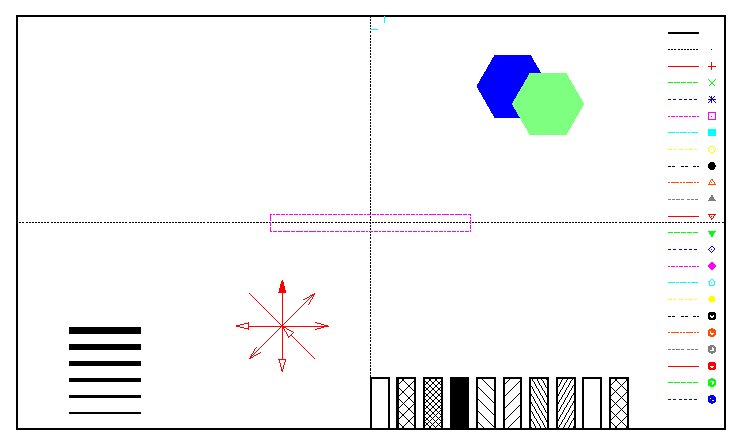
\includegraphics{GNUwykres-gnuplottex-fig3}}%
    \gplfronttext
  \end{picture}%
\endgroup
